\chapter{Implementation}

\section{Technologies}
\subsection{Kotlin Framework Ktor}

\subsection{Kotlin Library Ktorm}

\subsection{Koin}

Koin is a dependency injection framework that is available for the Kotlin programming language (https://insert-koin.io/). In this Application we use Koin to manage Objects like a Database object that is shared between asynchronous Route Objects and make it accessible.

\begin{minted}{kotlin}
val config = ConfigLoader().loadConfig()
val logger = LoggerFactory.getLogger("api")

startKoin {
    modules(
        org.koin.dsl.module {
            single { config }
            single(qualifier("main")) { config.databases.main }
            single { logger }
            single { BpmDatabase() }
            single { JwtConfig(config.token) }
        },
        RecommenderRoutes.koinModule()
    )
}
\end{minted}

\subsection{Ktor Plugins}

\subsubsection{CORS}

CORS or cross origin resource ... is a safety measure implemented in browsers to protect users ...

\subsubsection{Authentication}

For the authentication to access the different routes on the API Json Web Tokens or JWT is used. To configure this feature we also just install the authentication plugin with JWT.

\begin{minted}{kotlin}
fun Application.configureSecurity(jwtConfig: JwtConfig) {
    authentication {
        jwt {
            jwtConfig.configureKtorFeature(this)
        }
    }
}
\end{minted}

In this case more configuration is needed as we can save some data into the JWT to access this data within a request.

\subsubsection{Serialization}

The application uses JSON as Content Negotiation as defined in the functional requirements. The kotlin serialization plugin in combination with Ktorm enables the Application to send Kotlin Objects while the serialization plugin transform the objects to JSON and also transforms JSON within a http body to Kotlin object. 

\begin{minted}{kotlin}
fun Application.configureSerialization() {
    install(ContentNegotiation) {
        json()
    }
}
\end{minted}

\section{Architecture}

\subsection{Application Startup}

Application Startup ...

\newpage

\begin{figure}[h]
\centering
\includesvg{images/StartupBachelor.drawio.svg}
\caption{\label{fig:startup}description}
\end{figure}

\subsection{Routing}

\begin{figure}[ht]
\centering
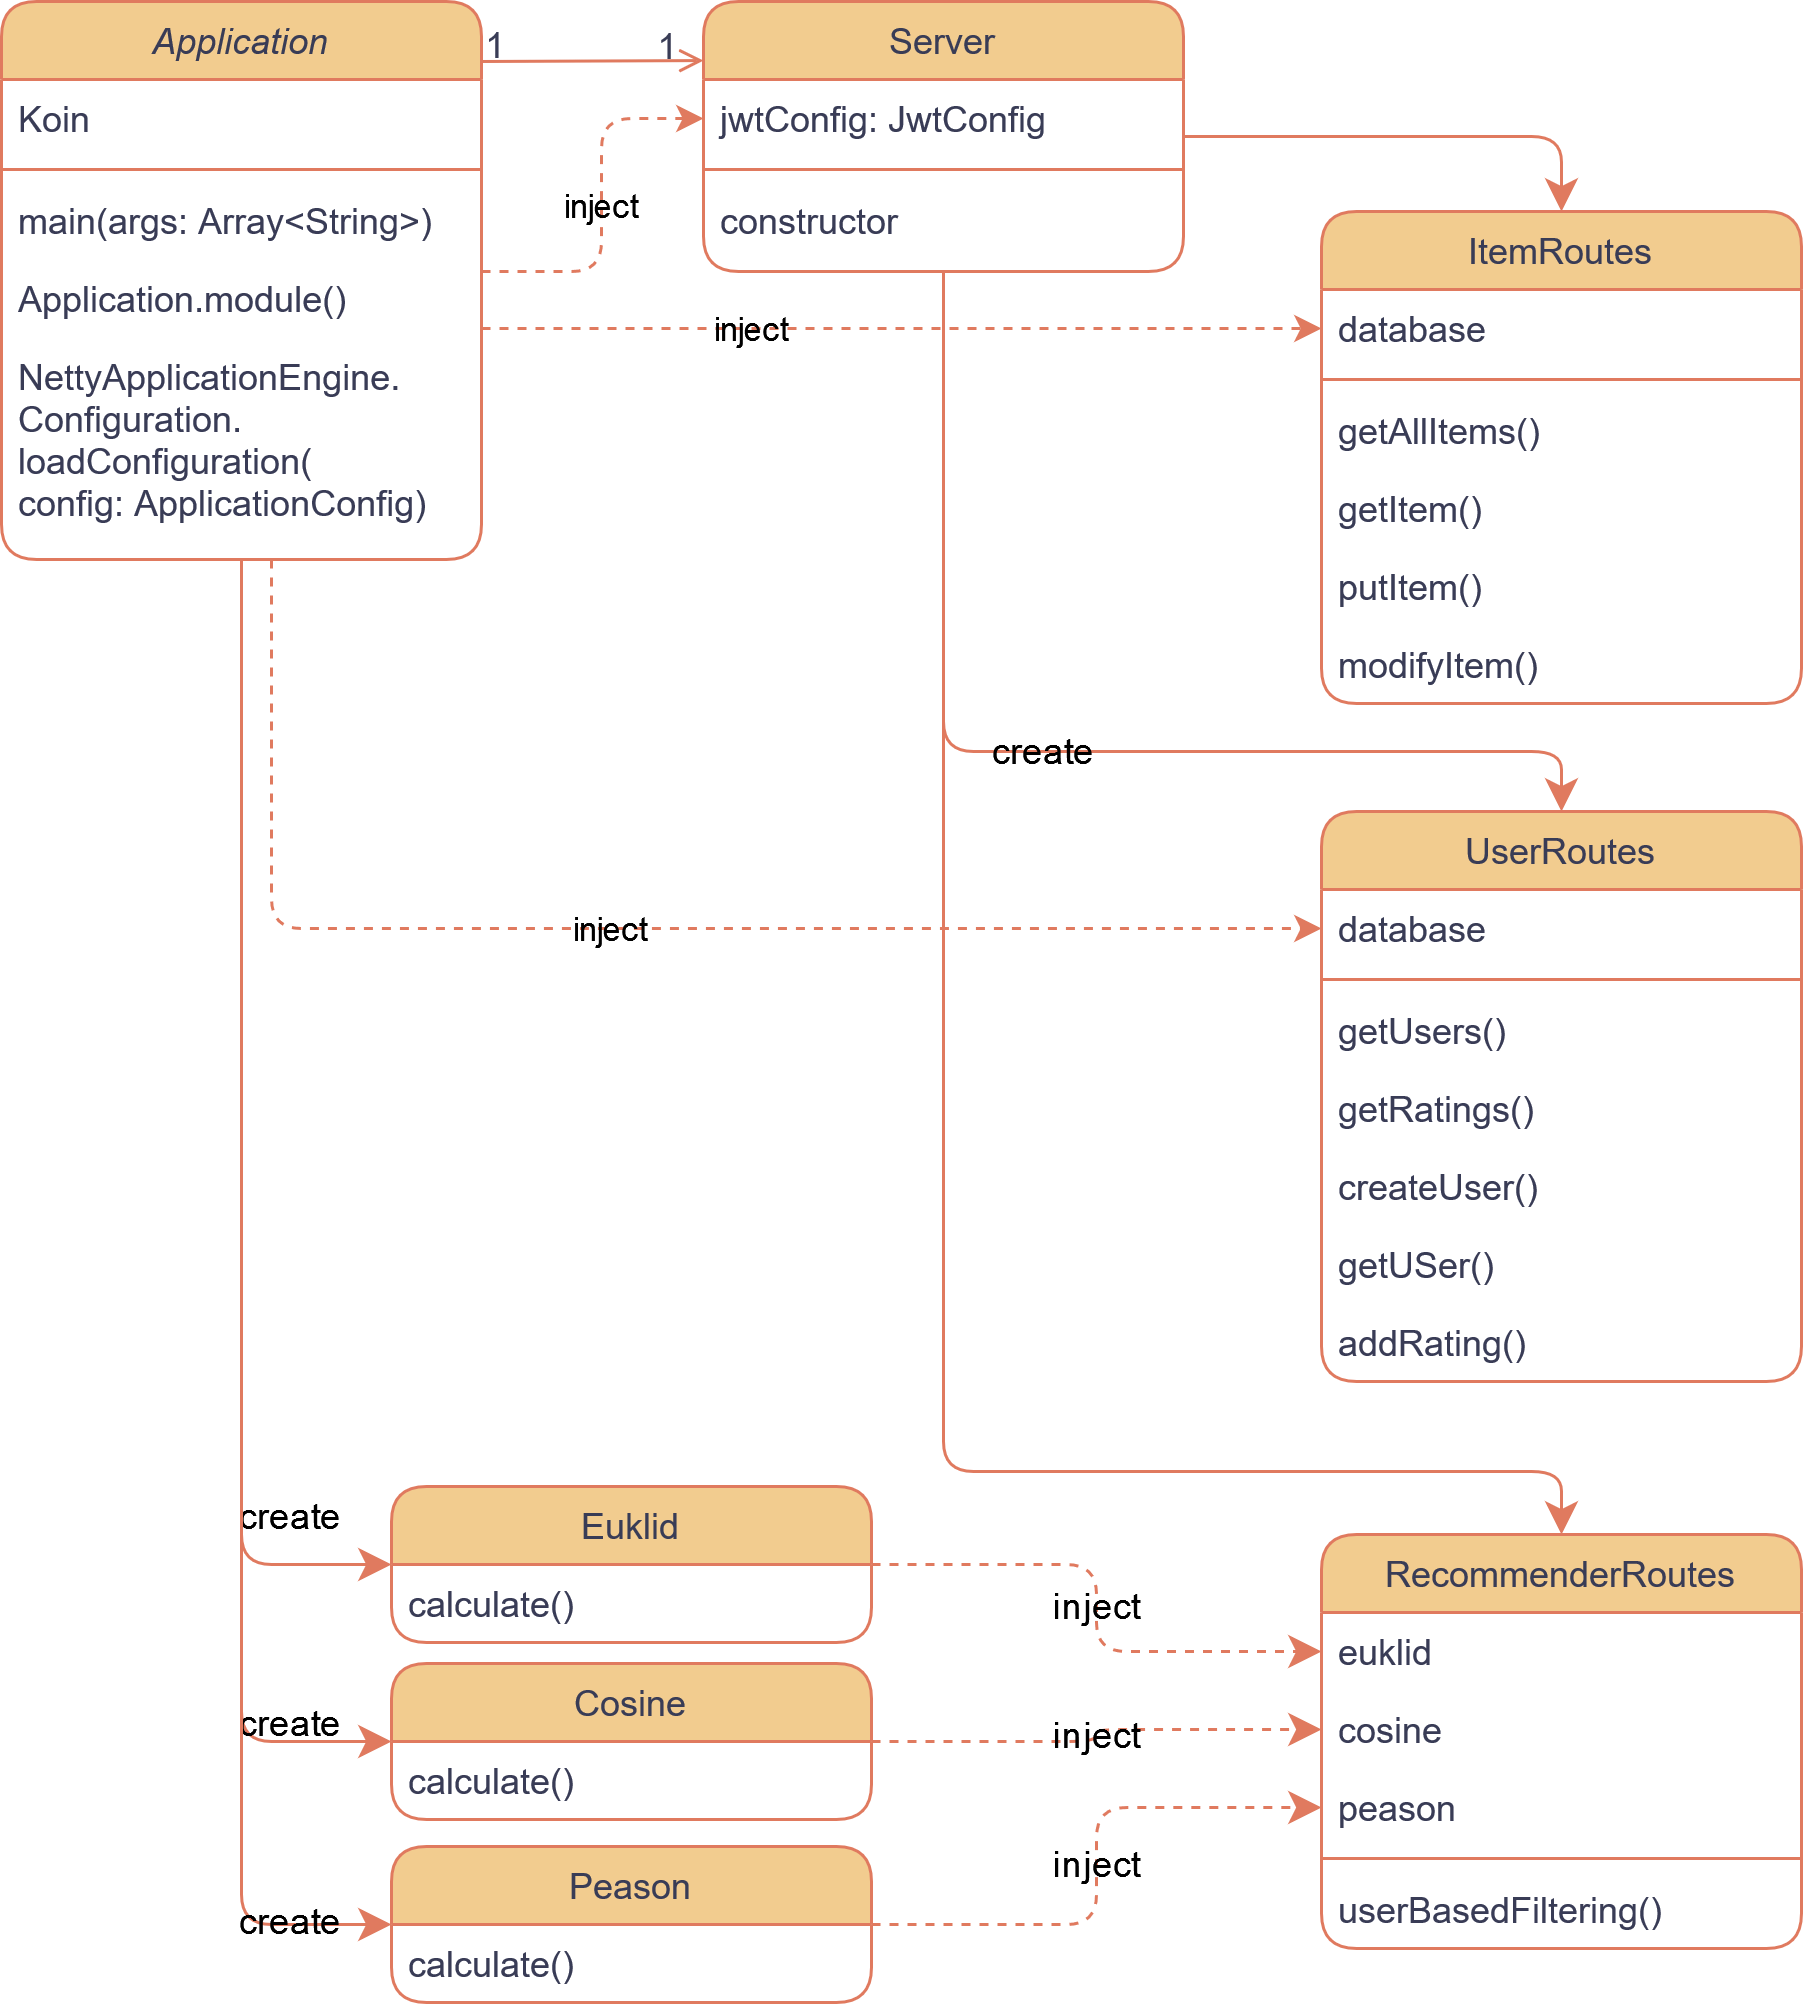
\includegraphics[width=\textwidth]{images/RoutingUML.png}
\caption{\label{fig:routing}Routing UML class diagram}
\end{figure}


\subsection{Database Access Objects}

\section{Recommendation Algorithms}

\subsection{Similarity Measures}

All similarity measures implement an Interface to facilitate the use of the algorithms.

\begin{minted}{kotlin}
interface SimilarityMeasure {
    /**
     * compares 2 data maps and returns a similarity measure,
     * note: comparing the result of this function only works 
     * with the same Similarity Measure!
     *
     * @param dataA the first data set
     * (key: the item, value: the rating of the item)
     * @param dataB the second data set
     * (key: the item, value: the rating of the item)
     * @param allItems all the items referenced in data1 & 2
     */
    fun compare(
        dataA: Map<String, Int>,
        dataB: Map<String, Int>,
        allItems: List<String>
    ): Number
}
\end{minted}

\subsubsection{Euclid}

The Euclidean Algorithm can calculate a similarity based on a distance. In other words if the distance between two users in small they are more similar. The dimension n is the item count.

\begin{equation}
S_{e} = \frac{1}{1+\sqrt{\sum_{i=1}^{n}{(dataA_i - dataB_i)^2}}}
\label{euklid}
\end{equation}

DataA and DataB refer to the ratings of two different users or items.
The implementation in Kotlin looks like this:

\begin{minted}{kotlin}
class Euclid : SimilarityMeasure {
    override fun compare(
        dataA: Map<String, Int>,
        dataB: Map<String, Int>,
        allItems: List<String>,
    ): Number {
        val sum = allItems.sumOf {
            ((dataA[it] ?: 0) - (dataB[it] ?: 0))
                .toDouble().pow(2)
        }

        return 1 / (1 + sqrt(sum))
    }
}
\end{minted}

The difference of the ratings of DataA and DataB is an Integer but is transformed into a double as the pow() function in the kotlin standard library is only defined on floats and doubles.

\subsubsection{Cosine}

The basic calculation is separated into the companion object of the class as the calculation is also used by the Pearson distance measure. 

\begin{minted}{kotlin}
class Cosine : SimilarityMeasure {
    companion object {
        fun basicCalc(
            dataA: Map<String, Number>,
            dataB: Map<String, Number>,
            allItems: List<String>,
        ): Number {
            var sumATimesB = 0.0
            var sumASquared = 0.0
            var sumBSquared = 0.0

            allItems.forEach {
                sumATimesB += (dataA[it] ?: 0).toDouble() * (dataB[it] ?: 0).toDouble()
                sumASquared += (dataA[it] ?: 0).toDouble().pow(2)
                sumBSquared += (dataB[it] ?: 0).toDouble().pow(2)
            }

            return (sumATimesB / (sqrt(sumASquared * sumBSquared)))
        }
    }

    override fun compare(
        dataA: Map<String, Int>,
        dataB: Map<String, Int>,
        allItems: List<String>,
    ): Number {
        return basicCalc(dataA, dataB, allItems)
    }
}
\end{minted}

\subsubsection{Pearson}

\subsection{Knn}

\subsection{Mean}